\setlength{\LSTxleftmargin}{2ex}%
\setlength{\LSTxrightmargin}{0ex}%
\setcounter{LSTcounterCharsPerLineOfCode}{86}%
%
\makeatletter%
\setlength{\LSTbasewidth@tmp}{\textwidth}%
\addtolength{\LSTbasewidth@tmp}{-\LSTxleftmargin}%                   xleftmargin
\addtolength{\LSTbasewidth@tmp}{-\LSTxrightmargin-\LSTxleftmargin}% compensation
\addtolength{\LSTbasewidth@tmp}{0.75ex}%        approx width of a-z in this font
\setlength{\LSTbasewidth}{\LSTbasewidth@tmp/\theLSTcounterCharsPerLineOfCode}%
\makeatother%
%
\lstset{%
xleftmargin=\LSTxleftmargin,%
xrightmargin=\LSTxrightmargin,%
basewidth=\LSTbasewidth%
}%
%
\colorlet{LSTcolorKeyword}{orange}%                 for, if, end, continue, etc.
%

% Useful macros:
\newcommand{\initModels}{\texttt{initModels}}
\newcommand{\twoTank}{\texttt{twoTank.py}}
\newcommand{\workflowfile}{\texttt{workflow}}
\newcommand{\FireTask}{\texttt{FireTask}}
\newcommand{\SurrogateFunction}{\textsf{SurrogateFunction}}
\newcommand{\classSurrogateModel}{\textsf{SurrogateModel}}
\newcommand{\FlowRateExactSim}{\textsf{FlowRateExactSim}}
\newcommand{\BackwardMappingModel}{\textsf{BackwardMappingModel}}
\newcommand{\ModenaBackwardMappingTask}{\textsf{ModenaBackwardMappingTask}}
\newcommand{\CFunction}{\texttt{CFunction}}
\newcommand{\LaunchPad}{\texttt{LaunchPad}}
\newcommand{\FireWorks}{\textsf{FireWorks}}
% from database.tex
% \newcommand{\fwname}{\texttt{\_fw\_name}}
% \newcommand{\surrogateModel}{\texttt{surrogate\_model}}
% \newcommand{\surrogateFunction}{\texttt{surrogate\_function}}
% \newcommand{\pZero}{\texttt{p0}}
% \newcommand{\rhoZero}{\texttt{rho0}}
% \newcommand{\pOneByPzero}{\texttt{p1Byp0}}
% \newcommand{\diameter}{\texttt{D}}
% \newcommand{\id}{\texttt{\_id}}
% \newcommand{\cls}{\texttt{\_cls}}
% \newcommand{\inputs}{\texttt{inputs}}
% \newcommand{\outputs}{\texttt{outputs}}
% \newcommand{\fitData}{\texttt{fitData}}
% \newcommand{\Min}{\texttt{min}}
% \newcommand{\Max}{\texttt{max}}
% \newcommand{\argPos}{\texttt{argPos}}
% \newcommand{\params}{\texttt{parameters}}
% \newcommand{\paramOne}{\texttt{param1}}
% \newcommand{\paramTwo}{\texttt{param2}}
% \newcommand{\flowRate}{\texttt{flowRate}}
% \newcommand{\libraryName}{\texttt{libraryName}}
% \newcommand{\functionName}{\texttt{libraryName}}
% \newcommand{\Ccode}{\texttt{Ccode}}
% \newcommand{\exactTask}{\texttt{exactTask}}
% \newcommand{\inheritedInputs}{\texttt{inherited\_inputs}}
% \newcommand{\initializationStrategy}{\texttt{initializationStrategy}}
% \newcommand{\outofBoundsStrategy}{\texttt{outofBoundsStrategy}}
% \newcommand{\ParameterfittingStrategy}{\texttt{ParameterfittingStrategy}}
% \newcommand{\improveErrorStrategy}{\texttt{improveErrorStrategy}}
% \newcommand{\initialPoints}{\texttt{initialPoints}}
% \newcommand{\nSamples}{\texttt{nSamples}}
% \newcommand{\nNewPoints}{\texttt{nNewPoints}}
% \newcommand{\maxerror}{\texttt{maxerror}}
% \newcommand{\maxIterations}{\texttt{maxIterations}}
% \newcommand{\testDataPercentage}{\texttt{testDataPercentage}}
% \newcommand{\outsidePoint}{\texttt{outsidePoint}}
% \newcommand{\surrFunction}{\texttt{surrogateFunction}}
% \newcommand{\tst}{\texttt{test}}
% \newcommand{\lcl}{\texttt{local}}
% \newcommand{\fireworks}{\texttt{fireworks}}
% \newcommand{\sysIndex}{\texttt{system.indexes}}
% \newcommand{\catOne}{\texttt{cat\_1.}}

%%%%%%%%%%%%%%%%%%%%%%%%%%%%%%%%%%%%%%%%%%%%%%%%%%%%%%%%%%%%%%%%%%%%%%%%%%%%%%
%                               Main Sections                                %
% ========================================================================== %
%                                                                            %
%                                                                            %

% ------------------------------- Section ---------------------------------- %
%%                                                                          %%
%%%                                                                        %%%
%%                                                                          %%
% -------------------------------------------------------------------------- %
\section{Testing on two tank example}
\label{sec:twoTanks}
% .......................................................................... %
%%                                                                          %%
% .......................................................................... %
\subsection{Physical Description}
%
\begin{figure}
  \centering
  \includegraphics[width=0.5\textwidth,keepaspectratio=true]{./Content/Figures/twoTanks.pdf}
  \caption{Schematic representation of the two tank example.}
  \label{fig:twoTanks}
\end{figure}

"Two tanks" is a basic example designed to show the structure of the framework using a simple model of the discharge of air from one tank into another through a nozzle is considered as depepicted in Figure \ref{fig:twoTanks}. 
In order for the example to makes sense from a {\MoDeNa} perspective, the flow through the nozzle must be considered as a complex problem which that has to be solved using 3D {\ComputationalFluidDynamics} or a different detailed model. 
Consequently, the two tanks are macroscopic models and the rate of discharge of fluid through the nozzle represents a microscopic model. 
Moreover, the example also demonstrates a backward mapping problem if the range of the inputs is assumed to be unknown apriori. 
%
\par
%
In the example, the dynamic simulation, describing the contents of the two tanks, uses the {\MoDeNa} interface library to embed a surrogate model describing the rate of discharge of fluid through the nozzle. 
In other words, the file \texttt{twoTanksMacroscopicProblem.C} is the macroscopic scale. 
The microscopic scale, a detailed model describing the dischage of fluid, is implemented in \texttt{twoTanksFullProblem.C}. 
The latter is never explicitly executed by the macroscopic code, but through the {\MoDeNa} framework when the surrogate model is out of bounds. 
%
\par
%
The micro scale model, shown in equation \ref{eq:nozzleEquation}, was obtained from \cite{VDI}.
\begin{equation}
    \HeatFlow = \pi \Diameter^2 \ValveConstant \ThermodynamicConstant \sqrt{ 2 \Pressure_1 \Density{}} \label{eq:nozzleEquation}
\end{equation}
The variables of model, $\Pressure_1$ and $\Pressure_2$ describes the pressures in Tank 1 and Tank 2, respectively. 
{\Diameter} is the diameter of the nozzle and {\Density{}} is the density of the fluid (air).
The model parameters shown below are respectively an empirical correlation and derived from thermodynamic assumptions.
\begin{align*}
\ValveConstant &= 0.84-
      0.66 \displaystyle{ \left( \frac{\Pressure_2}{\Pressure_1} \right) }^2 +
      0.48 \displaystyle{ \left( \frac{\Pressure_2}{\Pressure_1} \right) }^3 \\
      %
\ThermodynamicConstant &= 
      \sqrt{\displaystyle\left(
                             \frac{\CpOverCv}{\CpOverCv-1}
                         \right)
            \displaystyle{\left(
                             \frac{\Pressure_2}{\Pressure_1}
                         \right)}^{2/\CpOverCv} -
            \displaystyle{\left(
                             \frac{\Pressure_2}{\Pressure_1}
                          \right)}^{\frac{\CpOverCv +1 }{\CpOverCv}}} 
     &; \CpOverCv = \CpOverCv^{\text{air}} = 1.4
\end{align*}
The surrogate model approximating the detailed model in equation \ref{eq:nozzleEquation} is shown in equation (\ref{eq:surrogateModel}).
\begin{equation}
    \widetilde{\HeatFlow} = 
    \pi \Diameter^2 \SurrogateParameter_2 
    \sqrt{ \SurrogateParameter_1 \Density{} \Pressure_1}
    \label{eq:surrogateModel}
\end{equation}
The parameters, $\SurrogateParameter_1$ and $\SurrogateParameter_2$, in the surrogate model are degrees of freedom used in order to approximate the detailed model in equation \ref{eq:nozzleEquation}.
%
\par
%
The surrogate model is not explicitly defined in the file, \texttt{twoTanksMacroscopicProblem.C}, but the simulation can access the model from {\MongoDB} using the {\MoDeNa} syntax.
Additionally, the file contains the initial conditions and dynamic equations describing the behaviour of the two tank system. 
When the simulation is startet it will therefore look for a surrogate model \texttt{flowRate} in the database and start solving the differential equations. 
%
\par
%
The initial conditions are defined as follows:
\begin{itemize}
 \item Pressure in Tank 1 = 300000 Pa
 \item Pressure in Tank 2 = 10000 Pa
 \item Volume of Tank 1 = 0.1 L
 \item Volume of Tank 2 = 1 L
 \item Temperature of the system = 300 K (assumed constant)
\end{itemize}
%
When the surrogate model is used out of bounds, the {\MoDeNa} framework steps inn and extends the range in which the surrogate can be used before the simulation is allowed to continue.
%
\par
%
However, in order for the simulation to work the surrogate model has to be defined and put into the database. 
This procedure is described in Subsection \ref{subsec:initialization} and in short consists of defining two items:
\begin{description}
    \item[surrogate function] the surrogate model computer code
    \item[surrogate model] contains a surrogate function as well as strategies for events, e.g. initialization. 
\end{description}
The nozzle surrogate model was initialised with the following values of the design variables:
\begin{itemize}
	\item $\Diameter: [0.01, 0.01, 0.01, 0.01]$
	\item $\Density{}: [3.4, 3.5, 3.4, 3.5]$
	\item $\Pressure_1: [280000, 320000, 280000, 320000]$
	\item $\Pressure_2/\Pressure_1: [0.03, 0.03, 0.04, 0.04]$
\end{itemize}
%
The initialisation strategy determines how the surrogate model parameters $\SurrogateParameter_1$ and $\SurrogateParameter_1$ are determined.
When the initialisation is complete the surrogate model can be used by the macroscopic model. 
%
\par
%
\newcommand{\sunshine}{\ensuremath{\Time = 0.001}}
The macroscopic simulation is started as a firetask and solves the differential equation using a timestep of {\sunshine} seconds.
It calls the surrogate model at every timestem in order to calculate how much mass is discharged through the nozzle.
Afterwards, the ideal gas equation is used in order to update the pressure in the vessels due to the change in mass.
%
\par
%
It is during the evaluation of the surrogate model that the surrogate model may be used outside the range in which the parameters where initially determined. 
This causes the simulation to throw an exception telling the framework that the design space of the surrogate model is extended.
Consequently, the model is automatically updated by the {\MoDeNa} using the strategies that was specified when the model was defined. 
%
\par
%
This the simulation is paused while the surrogate model is updated, and starts from the beginning when the new parameters are fitted. 
The final result in Figure \ref{fig:twoTanks:Pressure} shows how the pressure of the tanks varies with respect to time.
From the complete simulation results it is not possible to see that the macroscopic model used a surrogate model that was fitted and re-fitted.
%
\begin{figure}
  \centering
  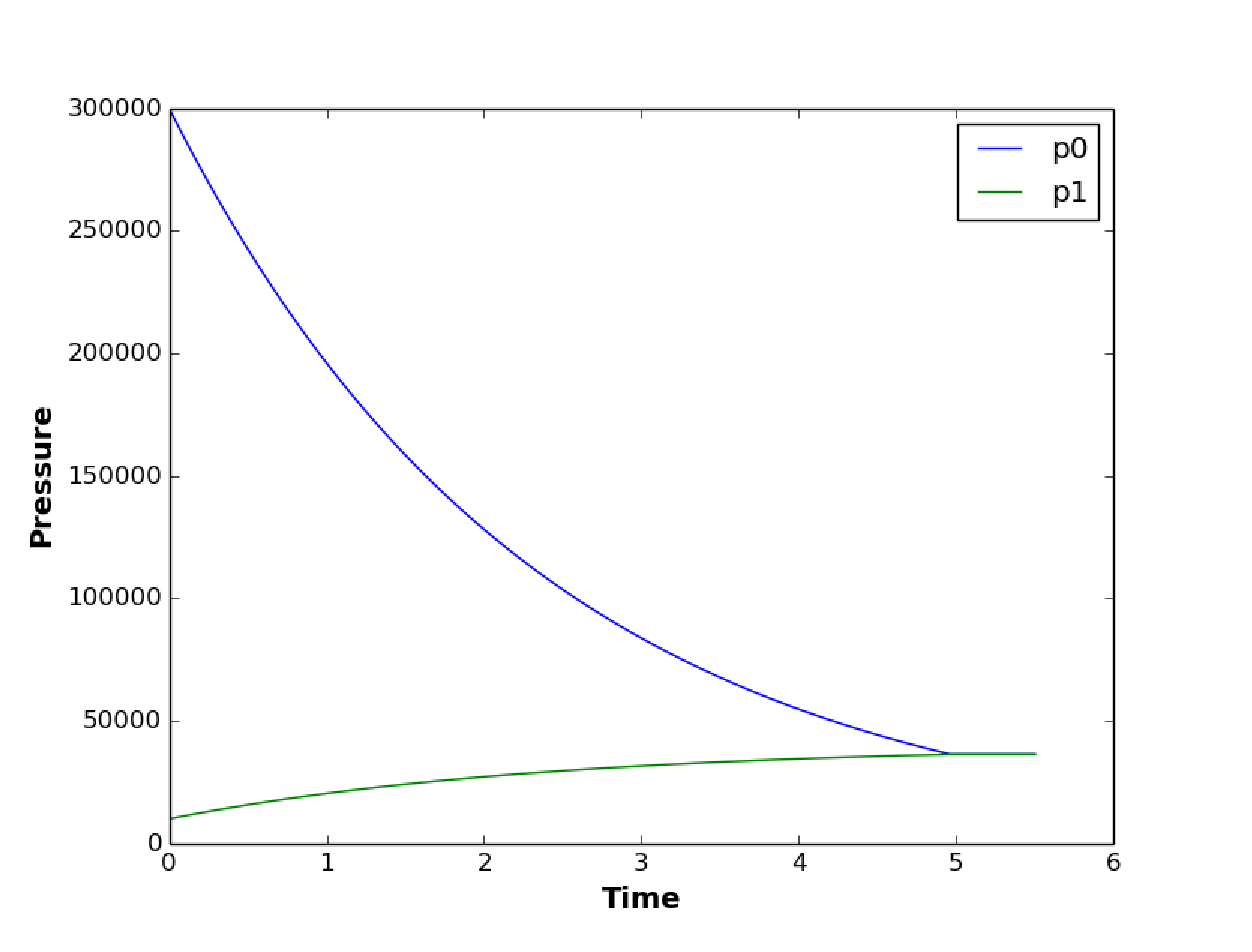
\includegraphics[width=0.5\textwidth,keepaspectratio=true]{./Content/Figures/pressureplot.eps}
  \caption{Pressures in the two tanks as a function of time.}
  \label{fig:twoTanks:Pressure}
\end{figure}
%
In order to show that the parameters in equation \ref{eq:surrogateModel} are changing dynamically throughout the simulation, Figure \ref{fig:twoTanks:Params} shows how the value of the parameters change with respect to the iteration number. 
This is helpful especially in identifying parts of the design space where the surrogate model provides a good approximation.
%
\begin{figure}
  \centering
  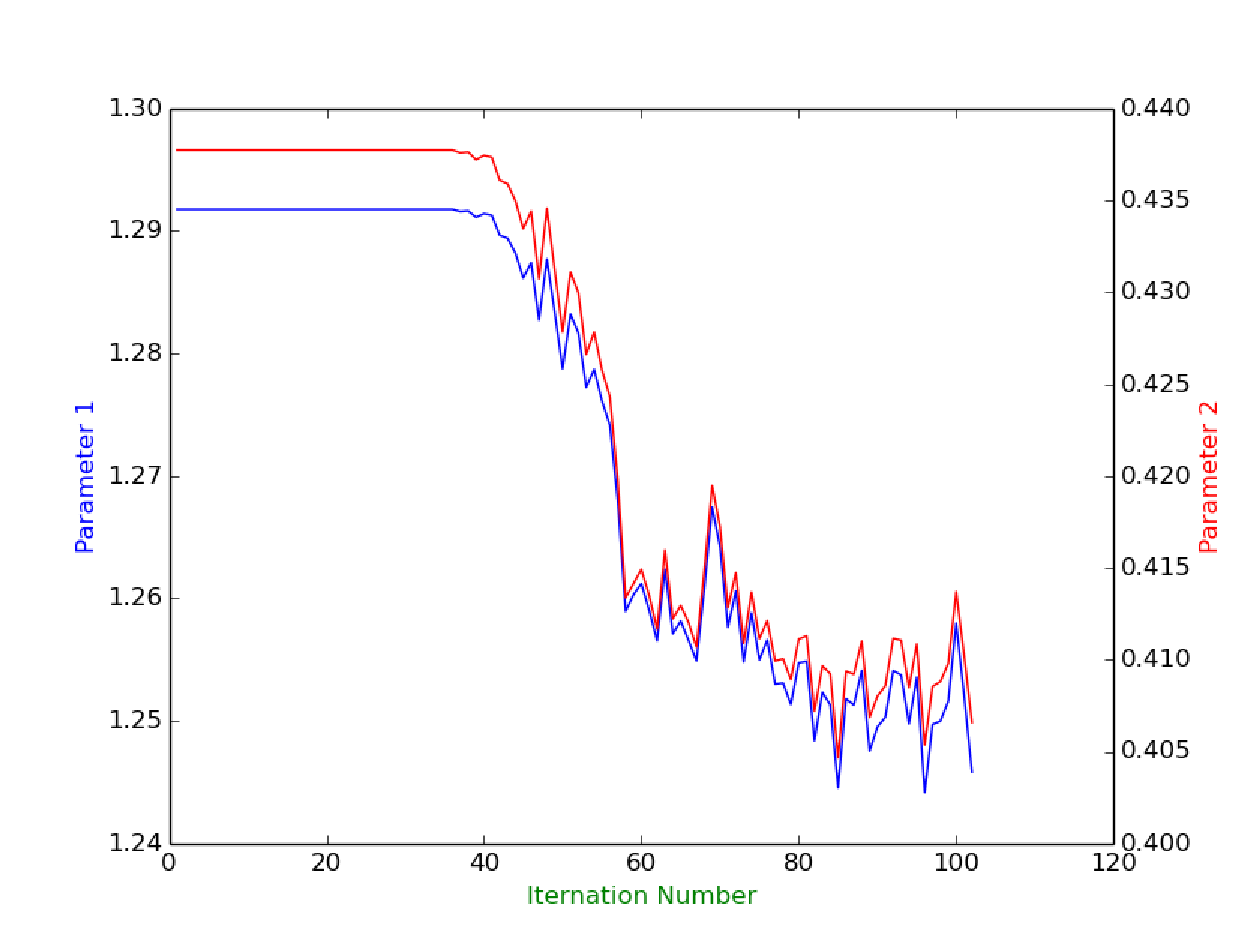
\includegraphics[width=0.5\textwidth,keepaspectratio=true]{./Content/Figures/plotparams.eps}
  \caption{Model parameters as function of backward mapping iterations.}
  \label{fig:twoTanks:Params}
\end{figure}
%
The introduction gave an overview ot the example and how the framework facilitates the simulation to be performed in a multi-scale, {\MoDeNa}-equivalent manner. 
The next sections aims at describing the code initiating and performing the parts of the simulation specific to the {\MoDeNa}-framework.
% .......................................................................... %
%%                                                                          %%
% .......................................................................... %
\subsection{Initialization}
    \label{subsec:initialization}
%
The {\initModels} script handles the initialization of the twoTank example.
First, the relevant \textcolor{blue}{classes} and \textcolor{cyan}{functions} from the {\MoDeNa} interface library, as well as {\FireWorks}, are imported. 
%
%
\begin{lstlisting}[style=lstPython, firstnumber=42]
from modena import ForwardMappingModel, BackwardMappingModel, SurrogateModel, CFunction
import modena.Strategy as Strategy
import twoTank
from fireworks import Firework, Workflow, LaunchPad
from fireworks.core.rocket_launcher import rapidfire
\end{lstlisting}
%
%The classes \lstinline[style=lstPython]{CFunction, ForwardMappingModel, BackwardMappingModel} are respectively used in order to create \lstinline[style=lstPython]{SurrogateFunction} and two different kinds of \lstinline[style=lstPython]{SurrogateModel} \textbf{objects}.
%
\par
%
The code block below shows how surrogate functions contains raw {\Clang}-code. 
The code is automatically compiled and prepared for use, the reason it can be used by the macroscopic models is that the mandatory fields \emph{inputs}, \emph{outputs} and \emph{parameters} can be accessed by the macromodels through adaptors. 
%
\begin{lstlisting}[style=lstPython, firstnumber=49]
f = CFunction(
    Ccode= '''
#include "modena.h"
#include "math.h"

void two_tank_flowRate
(
    const double* parameters,
    const double* inherited_inputs,
    const double* inputs,
    double *outputs
)
{
    const double D = inputs[0];
    const double rho0 = inputs[1];
    const double p0 = inputs[2];
    const double p1 = p0*inputs[3];

    const double P0 = parameters[0];
    const double P1 = parameters[1];

    outputs[0] = M_PI*pow(D, 2.0)*P1*sqrt(P0*rho0*p0);
}
''',
    # These are global bounds for the function
    inputs={
        'D': { 'min': 0, 'max': 9e99, 'argPos': 0 },
        'rho0': { 'min': 0, 'max': 9e99, 'argPos': 1 },
        'p0': { 'min': 0, 'max': 9e99, 'argPos': 2 },
        'p1Byp0': { 'min': 0, 'max': 1.0, 'argPos': 3},
    },
    outputs={
        'flowRate': { 'min': 9e99, 'max': -9e99, 'argPos': 0 },
    },
    parameters={
        'param0': { 'min': 0.0, 'max': 10.0, 'argPos': 0 },
        'param1': { 'min': 0.0, 'max': 10.0, 'argPos': 1 },
    },
)
\end{lstlisting}
%
%The reason the terminology surrogate function was used for the \lstinline[style=lstPython]{CFunction} class is that it is an instance of the \emph{parent class} {\SurrogateFunction}. 
The reason for the \texttt{CFunction} name is \emph{syntactic sugar} making it possible to provide flexibility for the user to specify surrogate models in different programming languages. 
The inputs, outputs and parameter dictionaries - which contain the minimum, maximum and the argument positions of the corresponding design variables or parameters - are also stored in the database collection as key and value pairs.
The creation of a surrogate function automatically updates the collection surrogate function in {\MongoDB}, as explained in Section \ref{sec:database}.
%
\par
%
When a surrogate function is saved in the database it is ready to be used in a surrogate model.
%There are two subclasses, \lstinline[style=lstPython]{ForwardMappingModel} and \lstinline[style=lstPython]{BackwardMappingModel}, of the parent class \lstinline[style=lstPython]{SurrogateModel}. 
The code block below shows how the backward mapping model in the two tanks example is defined in \texttt{initModels}.
%
\begin{lstlisting}[style=Python, firstnumber=89]
m = BackwardMappingModel(
    _id= 'flowRate',
    surrogateFunction= f,
    exactTask= twoTank.FlowRateExactSim(),
    substituteModels= [ ],
    initialisationStrategy= Strategy.InitialPoints(
        initialPoints=
        {
            'D': [0.01, 0.01, 0.01, 0.01],
            'rho0': [3.4, 3.5, 3.4, 3.5],
            'p0': [2.8e5, 3.2e5, 2.8e5, 3.2e5],
            'p1Byp0': [0.03, 0.03, 0.04, 0.04],
        },
    ),
    outOfBoundsStrategy= Strategy.ExtendSpaceStochasticSampling(
        nNewPoints= 4
    ),
    parameterFittingStrategy= Strategy.NonLinFitWithErrorContol(
        testDataPercentage= 0.2,
        maxError= 0.05,
        improveErrorStrategy= Strategy.StochasticSampling(
            nNewPoints= 2
        ),
        maxIterations= 5 # Currently not used
    ),
)
\end{lstlisting}
%
An instance of the {\classSurrogateModel} class is created with: the model {\id}, the base surrogate function, described previously, {\FlowRateExactSim} from {\twoTank}, which calls the {\exactTask} of the twoTank example, and the various strategies.
It is the surrogate model that is referenced to by the simulation in \texttt{twoTanksMacroscopicProblem.C}. 
The model is found in the database by looking up the {\id} in the surrogate models collection described in Section \ref{sec:database}.
Consequently, if the model has not been instantiated the simulation fails. 
Moreover, the framework will throw an error if the mandatory strategies, e.g.  {\outofBoundsStrategy} and the {\ParameterfittingStrategy}, have not been set. 
All the strategies are classes defined in the source file \emph{Strategies.py}.
%
\par
%
%The final code block in \texttt{initModels} performs the initialisation by executing the initialisation firework (\lstinline[style=lstPython]{.initialisationFw}) for all the objects of instance  surrogate model (\lstinline[style=lstPython]{m}) in the scope. 
%
\begin{lstlisting}[style=lstPython, firstnumber=117]
# set up the LaunchPad and reset it
launchpad = LaunchPad()
launchpad.reset('', require_password=False)

initFws = []
for m in SurrogateModel.get_instances():
    initFws.append(m.initialisationFw())

# store workflow and launch it locally
launchpad.add_wf(Workflow(initFws, {}, name="initialisation"))
rapidfire(launchpad)
\end{lstlisting}
%In the codeblock the surrogate models are put into the Fireworks (\lstinline[style=lstPython]{launchpad}), a server that manages Workflows, is reset so that it can be loaded with the Fireworks.
%The function \lstinline[style=lstPython]{rapidfire} tells fireworks to execute the workflow in the most convenient order.
Afterwards, the surrogate models are ready to be used and the simulation can be started.
% .......................................................................... %
%%                                                                          %%
% .......................................................................... %
\subsection{\twoTank}
%
The {\twoTank} file contains the two {\FireTask}s that start the microscopic and the macroscopic codes.
This file explicitly defines {\FireTask}, this was not done for the surrogate models because they already are defined to be firetasks, but it is hidden from the user for convenience reasons. 
The result is that the imported modules in {\twoTank} are different to those in \texttt{initModels}. 
%
\begin{lstlisting}[style=lstPython, firstnumber=39]
import os
import modena
from fireworks.user_objects.firetasks.script_task import FireTaskBase, ScriptTask
from fireworks import Firework, Workflow, FWAction
from fireworks.utilities.fw_utilities import explicit_serialize
from blessings import Terminal
\end{lstlisting}
%
The necessary imports are the {\MoDeNa} interface library, relevant objects from {\FireWorks} and a python package providing colored terminal output.
%
\par
%
The file defines two firetasks, the first executing the microscopic model and the second executing the macroscopic, both of which are compiled {\Clang} files.
%The microscopic model below prints the input to the code into a \texttt{.txt} file, executes the code (\lstinline[style=lstPython]{os.system('../src/flowRateExact')}) and picks up the output from a second \texttt{.txt} file made by the model.
%Afterwards, it returns a {\FireTask} that updates the database of the model (\lstinline[style=lstPython]|FWAction(mod_spec=[{'_push': self['point']}])|).
%
\begin{lstlisting}[style=lstPython, firstnumber=59]
@explicit_serialize
class FlowRateExactSim(FireTaskBase):
    """
    A FireTask that starts a microscopic code and updates the database.
    """

    def run_task(self, fw_spec):
        print(
            term.yellow
          + "Performing exact simulation (microscopic code recipe)"
          + term.normal
        )

        D = self['point']['D']
        rho0 = self['point']['rho0']
        p0 = self['point']['p0']
        p1Byp0 = self['point']['p1Byp0']

        # Write input
        f = open('in.txt', 'w')
        f.write('%g\n%g\n%g\n%g\n' % (D, rho0, p0, p1Byp0))
        f.close()

        # Execute the application
        # In this simple example, this call stands for a complex microscopic
        # code - such as full 3D CFD simulation.
        # Source code in src/flowRateExact.C
        os.system('../src/flowRateExact')

        # Analyse output
        f = open('out.txt', 'r')
        self['point']['flowRate'] = float(f.readline())
        f.close()

        return FWAction(mod_spec=[{'_push': self['point']}])
\end{lstlisting}
%
The second {\FireTask} starts the macroscopic code at the following command:
\\ 
%\lstinline[style=lstPython]{ super(ModenaBackwardMappingTask, self).run_task(fw_spec) }
\\
However, unlike the microscopic firetask this can end in two ways:
\\
% \lstinline[style=lstPython]{return model.outOfBoundsFwAction(model,self,outsidePoint= model.outsidePoint)} 
\\
 or
\\
%\lstinline[style=lstPython]{return ret}
%
\begin{lstlisting}[style=lstPython, firstnumber=97]
@explicit_serialize
class ModenaBackwardMappingTask(ScriptTask):
    """
    A FireTask that starts a macroscopic code and catches its return code.
    @author: Henrik Rusche
    """
    required_params = ['script']

    def run_task(self, fw_spec):
        print(
            term.yellow
          + "Performing backward mapping simulation (macroscopic code recipe)"
          + term.normal
        )

        self['defuse_bad_rc'] = True

        # Execute the macroscopic code by calling function in base class
        ret = super(ModenaBackwardMappingTask, self).run_task(fw_spec)

        # Analyse return code

        print('return code = %i' % ret.stored_data['returncode'])
        if ret.stored_data['returncode'] > 199:
            print term.cyan + "Performing Design of Experiments" + term.normal
            model = modena.SurrogateModel.loadFailing()

            return model.outOfBoundsFwAction(
                model,
                self,
                outsidePoint= model.outsidePoint
            )

        else:
            print('We are done')
            return ret
\end{lstlisting}
%
The reason why the {\ModenaBackwardMappingTask} {\FireTask} has two possible outcomes is because it executes the \texttt{twoTanksMacroscopicProblem} code. 
The two outcomes represents starting design of experiments and parameter fitting, and terminating the entire workflow when the simulation is complete. 
%
\par
%
Simular to the exact simulation mentioned in the previous code bloc, the backward mapping {\FireTask} is a \texttt{ScriptTask}, which helps running non-Python scripts through the command line. 
The required parameter for this class is \texttt{script}. 
In the twoTank example, the \texttt{script} is an executable, i.e. compiled {\Clang}-code, representing the macroscopic  \texttt{twoTanksMacroscopicProblem}. 
%
\par
%
However, the workflow itself is initiated in the {\workflowfile} file shown below.
%
\begin{lstlisting}[style=lstPython, firstnumber=45]
# set up the LaunchPad and reset it
launchpad = LaunchPad()
launchpad.reset('', require_password=False)

# create the individual FireWorks and Workflow
# Source code in src/twoTanksMacroscopicProblem.C
fw1 = Firework(
    ModenaBackwardMappingTask(
        script='../src/twoTanksMacroscopicProblem'
    )
)
wf = Workflow([fw1], {}, name="simulation")

# store workflow and launch it locally
launchpad.add_wf(wf)
rapidfire(launchpad)
\end{lstlisting}
%
The {\LaunchPad} is reset so that it can be loaded with the Fireworks.
A Firework is created using the {\ModenaBackwardMappingTask} class through the macroscopic \texttt{script}.
A Workflow is then created using this Firework, added to the \textsf{Launchpad} and executed.
%
\par
%
The return code of this macroscopic \texttt{script} is caught in the {\ModenaBackwardMappingTask} class.
The return code indicates whether or not there is an {\outsidePoint}.
If there is, it returns the \texttt{outOfBoundsFwAction}, meaning that the Design of Experiments is performed.
If not, the simulation ends.
